\documentclass{article}
\usepackage[dutch]{babel}
\usepackage{graphicx}
\author{Sander Cleymans}
\date{\today}
\title{Ontwikkeling van Bedrijfstoepassingen \\
		Casestudie Ryanair}

\begin{document} 

\maketitle

\newpage  

\tableofcontents

\newpage
\part{Samenvatting voor de raad van Bestuur}

In dit verslag maak ik casestudie voor Ryanair in 2014.
Allereerst worden de algemene kenmerken van het bedrijf aangehaald, onder meer de concurrentie en de standpunten van Ryanair tegenover bepaalde 'vaste waarden' uit de industrie.
   
De concurrentie van Ryanair is door de jaren enkele keren verandert, maar een van de vaste waarden bij de Europese Low-Cost Carriers (LCC's) en een geduchte concurrent van Ryanair, is het Britse easyJet. Daarnaast is er natuurlijk nog de grote groep traditionele luchtvaartmaatschappijen die allemaal hun eigen doelpubliek hebben, maar allemaal vechten om de overgebleven klanten te kunnen overtuigen om bij hen te vliegen.
	
In het tweede stuk van het verslag ga ik iets dieper in op alle verschillende kritieke succesfactoren (CSF's) gerelateerd aan Ryanair:

\begin{itemize}
\item Trouw blijven aan de de point-to-point verbindingen die ze aanhouden met de secundaire(!) luchthavens.
\item De laagste prijs behouden.
\item Zoeken naar innovatieve concepten en vooruitstrevende manieren van denken
\item Klantgerichtheid
\end{itemize}

Bij elk van deze CSF's wordt er uitgelegd van waar deze komt en er worden er nog enkele andere aangehaald.
Hieruit is er een clustering analyse gedaan en verdere uitwerking naar een volledig schema, om de kernsystemen te kunnen vaststellen. Deze hebben we kunnen vastleggen als Quality control, Sales en Planning. Een value chain model en value chain network heb ik daarna opgesteld om te kunnen kijken naar wat nu essentieel is voor een groot bedrijf als Ryanair.

Het laatste deel over de informatie imperfecties is een beknopte terugblik naar wat er nu fout is aan de markt waarop Ryanair zich heeft geworpen, maar hoe het deze imperfecties naar het eigen voordeel kan aanwenden. Bounded Rationality en Opportunism moeten behouden blijven, Multi-interpretable information kan best verholpen worden om het bedrijf iets transparanter en toegankelijker te laten over komen.

\newpage
\part{Concurrentie en Competitie}

De huidige toestand van de luchtvaart-markt, laat ons toe om redelijk mooi in te schatten hoe sterk elke maatschappij zich heeft kunnen vestigen op een bepaalde plaats tegenover zijn onmiddellijke concurrenten.
Er is een duidelijk onderscheid te maken tussen de directe concurrenten en de indirecte concurrentie.

\section{Ryanair en easyJet}

De geschiedenis en de concurrentie tussen deze twee maatschappijen gaat terug tot het begin van de openstelling van het Europese luchtvaartindustrie in 1997. Momenteel zijn het nummer 1 en 2 op de Europese markt, maar daar is een heftige concurrentiestrijd aan vooraf gegaan. Omdat beide maatschappijen zich op dezelfde doelgroep richten (goedkope, point-to-point vluchten), trachten ze steeds de andere af te troeven op een bepaald vlak. Zij het om de prijzen voor een bepaalde route naar beneden te houden, zij het om het snelst uit te breiden naar nieuwe landen,...

Beide landen houden er dezelfde strategie op na: een no-frills, point-to-point vlucht aanbieden voor de laagst mogelijke prijs, zonder er zelf aan ten onder te gaan. Ze doen dit beide een zeer strak businessplan aan te houden: minimaal aantal verschillende vliegtuigtypes (bij Ryanair momenteel zelfs beperkt tot een type, de Boeing 737-800), alle extra's worden ook extra aangerekend en een beperkt aantal routes.

Een essentieel verschil tussen de twee is echter dat Ryanair zich strikt beperkt tot secundaire luchthavens, terwijl easyJet wel de grote aandoet: Paris Charles de Gaulle, London Gatwick, Brussels Airport en zowat elke andere grote Europese stad. Daar tegenover staat dat Ryanair (meestal) kleinere luchthavens aandoet: Brussel-Charleroi, Frankfurt-Hahn,... De laatste paar jaren zijn er hier echter enkele grotere bij gekomen. Dit omdat het zijn doelpubliek wil uitbreiden en in de running wil blijven met zijn grootste rivaal easyJet.\footnote{http://news.airwise.com/story/view/1385577015.html} Hierdoor wijkt het wel af van zijn eigen businessplan, maar met een goede verantwoording.

De strijd tussen de 2 heeft er voor gezorgd dat beide met enorm lage prijzen vluchten aanbieden naar zowat gans Europa (en enkele bestemmingen daarbuiten, maar voor dit verslag zullen we het bij Europa houden). Door hun geslaagde strategie zijn Ryanair en easyJet momenteel de twee grootste LCC's van Europa, met respectievelijk 81.4 en 59.2 miljoen passagiers in 2013.

\section{Andere concurrenten}

Hier komen we aan bij de andere concurrenten van Ryanair, waaronder we onder meer de vele kleine (veelal lokale) maatschappijen terugvinden, maar ook andere grote spelers op de markt: British Airways, Lufthansa, Iberia,... 
Het grootste verschil met Ryanair en easyJet is hier dat deze maatschappijen niet specifiek naar een low-budget model willen gaan. Zo worden, in tegenstelling met Ryanair (e.a.), zogenaamde 'ancillary services' niet extra aangerekend. Er wordt ook gevlogen naar grote luchthavens, men maakt gebruik van persoonlijk contact bij in/uitchecken van een vlucht en de boeking van een ticket, waar dat bij Ryanair zo goed als alles hiervan elektronisch gebeurd. Verder maken ze gebruik van een uitgebreidere vloot, wat hun iets meer vrijheid geeft over bezetting van vluchten en routes.
De routes van deze maatschappijen zijn ook van een andere soort, ze vertrekken meestal alleen uit hun thuisland, naar bepaalde bestemmingen (en terug natuurlijk). Dit in tegenstelling met Ryanair die bijvoorbeeld ook vluchten van Belgi\"e naar Frankrijk voorziet.

\part{Critical Success Factors van Ryan air}

Aangekomen bij ons volgend onderdeel van de bedrijfsanalyse, moeten we vaststellen welke CSF's er zijn voor het voorbestaan van het bedrijf. De strategie kan (heel rudimentair) herleid worden tot: De vlucht van punt A naar punt B moet zo goedkoop mogelijk zijn, zo vaak mogelijk vliegen en dat met de meeste passagiers.

\begin{enumerate}
\item De eerste en waarschijnlijk de belangrijkste van alle CSF's is dat Ryanair de goedkoopste luchtvaartmaatschappij blijft. Ryanair is momenteel de grootste binnen Europa, omdat het consistent de laagste prijs kan aanbieden voor de huidige routes. Moest een concurrent er in slagen dit te evenaren (of er onder gaan) en daarbij betere diensten te leveren, dan faalt het hele concept. 

Dit 'goedkoop zijn' kunnen we dus wel stellen als een CSF, waarvan de Informatie Items afgeleid kunnen worden:

\begin{itemize}
\item Maximaal gebruik van de beschikbare vliegtuigen. Zowel op vlak van aantal passagiers per vliegtuig, als in vliegtuigplanning. Een halfleeg vliegtuig of een vliegtuig dat lang stil staat, is een verliespost.
\item Fuel Hedging, door een gunstige prijs te kunnen te pakken te krijgen voor meerdere jaren, krijgt Ryanair een substanti\"ele voorsprong als de prijs plotseling heel hard fluctueert.
\item Opleiding personeel is slechts toegespitst op het hoognodige. Piloten moeten bijvoorbeeld slechts met 1 bepaald vliegtuigtype kunnen vliegen.
\item Gunstige deals met de luchthavens zorgen voor minder taksen en andere 'onnodige kosten'.
\end{itemize}

\item Een tweede succesfactor, is het trouw blijven aan de eigen strategie, die van de point-to-point verbindingen met de secundaire, kleinere luchthavens:

\begin{itemize}
\item Aantrekkelijke locaties die niet te ver van belangrijke plaatsen liggen.
\item Lagere kosten bij de lokale vliegvelden, door de grotere afstand en de mindere bezetting.
\item Kortere 'niet bruikbare' tijd van de vliegtuigen en personeel. Door de mindere bezetting van de vliegvelden, kunnen er meer vluchten vertrekken dan op drukke, grote vliegvelden. (Turnaround time)
\item Point-to-point verbindingen.
\end{itemize}

\item Door innovatieve beslissingen en vooruitstrevende concepten door te voeren heeft Ryanair zich sinds het begin kunnen vestigen als een geducht concurrent voor de traditionele luchtvaartmaatschappijen. De beslissing voor de uniforme vloot, het aanbieden van extra diensten/goederen tegen betaling en de reclame zijn slechts enkele voorbeelden.

\begin{itemize}
\item Het niet aanbieden van de gratis drankjes, de bagageservice,... heeft er voor gezorgd dat mensen die dat niet nodig vinden, hier ook niet voor moeten betalen en Ryanair moet hier dus niets voorzien. 
\item Door middel van het aanbieden van 'combo's' kunnen klanten hun vlucht ineens koppelen aan een hotel, een huurauto. Alles gemakkelijk bij elkaar zorgt dat klanten dit ook sneller doen en Ryanair haalt hier natuurlijk ook zijn centje uit.
\item Reclame op en binnen in het vliegtuig zorgden bij de introductie voor blikken van verbazing, maar zorgden wel voor een extra inkomstpost voor Ryanair.
\end{itemize}

\item Als een van de laatste CSF's zou ik ook nog de klanten willen aanbrengen. Zij zijn namelijk het grote doel van elke luchtvaartmaatschappij. Zij zorgen voor inkomsten en zijn net datgene dat van punt A naar punt B moet gebracht worden en dan nog zo snel mogelijk liefst ook.
\begin{itemize}
\item Bestemmingenkeuze wordt gedaan aan de hand van waar de klanten naartoe willen.
\item Publiciteit krijgen door (controversi\"ele) nieuwe concepten.
Een mooi voorbeeld hiervan is de CEO, Michael O'Leary. Volledig trouw aan het gezegde "There is no such thing as bad publicity"\footnote{http://www.phrases.org.uk/meanings/there-is-no-such-thing-as-bad-publicity.html \\
De zin wordt toegeschreven aan een zekere Phineas T. Barnum, maar er is geen betrouwbare bron beschikbaar} zorgt hij zo nu en dan met Ryanair voor controverse, wat zeker voor een naambekendheid heeft gezorgd.
\item Loyalty bonussen.
\item Verkoop van diensten en goederen.
\end{itemize}

Hierbuiten zijn er nog 2 andere CSF's, waarvoor ik de Information Items op dezelfde wijze heb afgeleid als bij de 4 voorgaande:
\item Personeel (flexibel,stressbestendigheid,productiviteit,..)
\item Klantenservice (online vertegenwoordiging, dienst na verkoop, up-to-date informatie,...)
\end{enumerate}


Met behulp van deze data stellen we een matrix op die alle dingen weergeeft (Ik heb nog extra Business Activities en Information items toegevoegd, zodat het uiteindelijke resultaat duidelijker zou worden, met het initi\"ele schema dat ik eerst had opgesteld was niet veel te doen\footnote{http://goo.gl/AxWDQM}). Dus met de nodige verbeteringen ben ik uiteindelijk tot bijgevoegd schema gekomen. Na het groeperen van alle C's en U's, kunnen we enkele groepen van CSF's afleiden.

\begin{figure}[h]
\centering
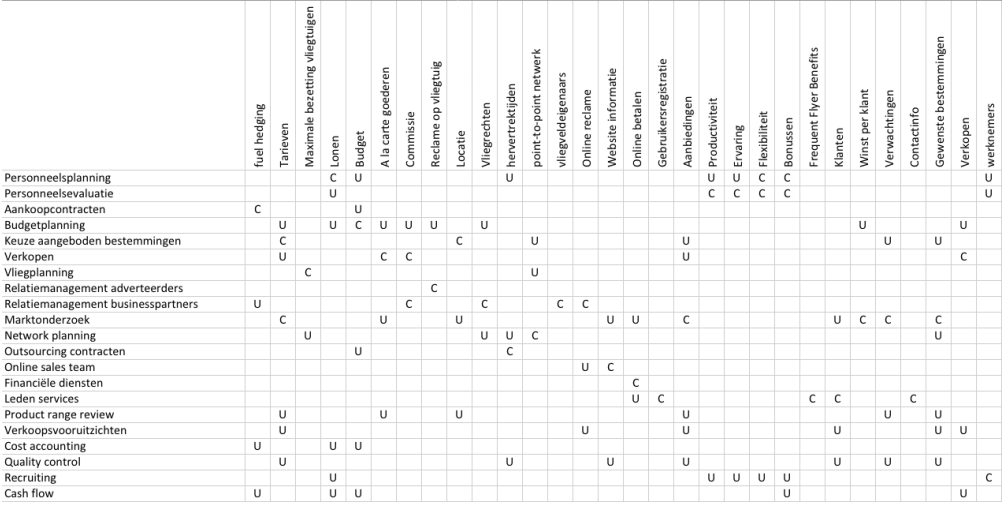
\includegraphics[scale=0.56]{image1}
\end{figure}
\begin{figure}[ht]
\centering
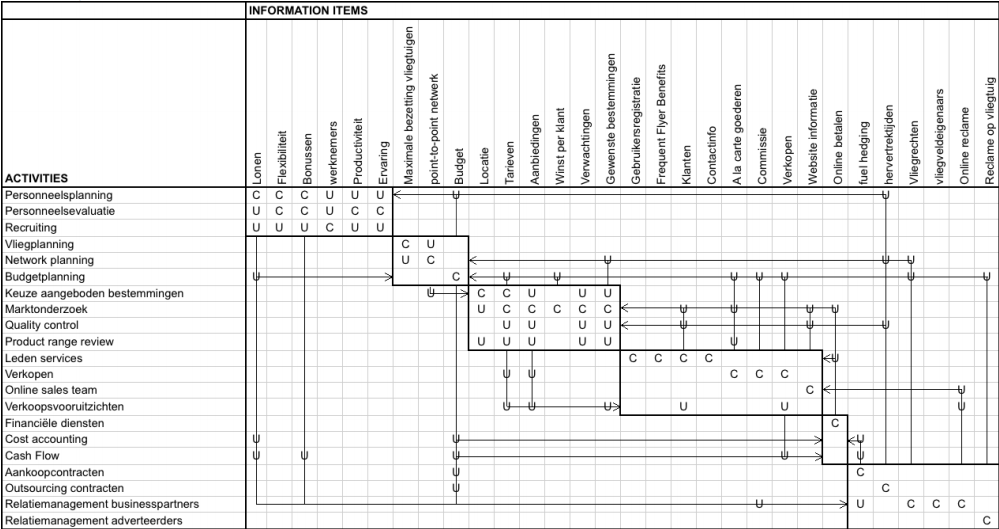
\includegraphics[scale=0.56]{image2}
\end{figure}
\begin{figure}[ht]
\centering
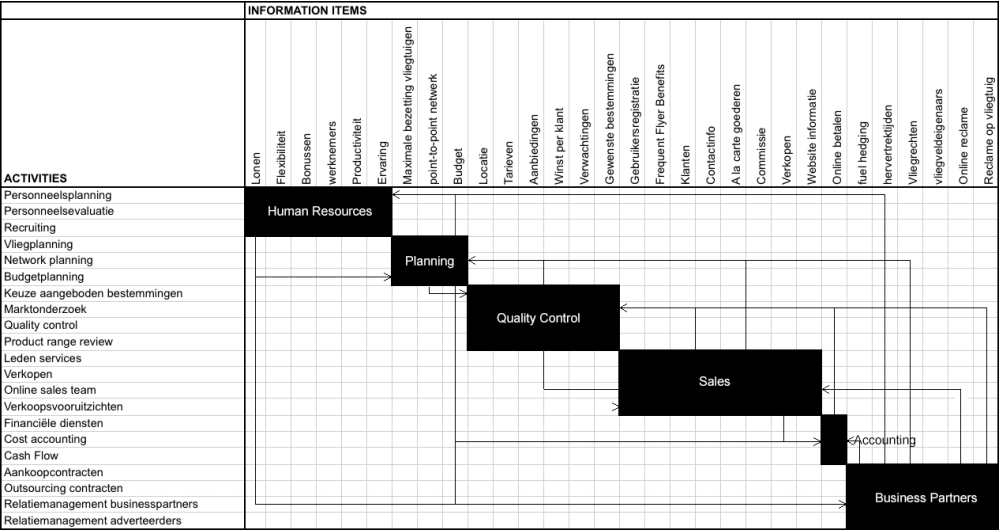
\includegraphics[scale=0.56]{image3}
\end{figure}


\newpage

De afbeeldingen laten zien dat er een 5-6 tal belangrijke systemen te onderscheiden zijn in Ryanair. Sales en Accounting zouden samen kunnen gaan tot een groter systeem, maar toch leek het me nuttig ze op te splitsen.

Quality control is een kernsysteem omdat Ryanair probeert te voldoen aan de standaarden die verwacht worden door de klanten. Ze zetten zichzelf niet zo zeer een vaste kwaliteitsstandaard voor, maar door een heel duidelijk marktonderzoek kunnen ze vaststellen wat de klanten verwachten. Door die vaststelling kunnen ze dan ontdekken waar en hoe de klant het liefst wordt voorzien van goede kwaliteitsproducten. Het is dan ook een van de dingen die bijdraagt aan de consistent lage prijs van de vluchten. Door op bepaalde (niet veelgevraagde) dingen, mindere kwaliteit te leveren, kunnen ze er voor zorgen dat de prijs voor het ticket naar een bepaalde bestemming (ook uit het marktonderzoek af te leiden) laag blijft.

Het tweede kernsysteem dat Ryanair hoog in het vaandel draagt, is Sales. Door het grote aanbod aan bestemmingen, de handige online aanwezigheid en de no-nonsense strategie slaagt Ryanair er in om zijn tickets snel en makkelijk te presenteren aan het grote publiek.

Een derde kernsysteem is de Planning. Ryanair zit momenteel met een enorm strakke planning. Hoge bezetting van routes, snelle turnaround time, een groot budget om goede deals met luchthavens binnen te halen, dragen allemaal bij tot een enorm goede planning. Evenals het feit dat ze de aankopen van nieuwe vliegtuigen altijd heel strategisch doen (crisistijd,...) wijst op een heel effici\"ente budgetplanning.

Deze drie systemen dragen bij tot wat Ryanair vandaag de dag de grootste van alle LCC's maakt. Gerichte kwaliteit, veel klanten en een goede (budgettaire) planning maken dat Ryanair ook de komende jaren waarschijnlijk de grootste zal blijven.

\part{Value Chain Model en Value Chain Network}
\setcounter{section}{0}
\section{Value Chain Model}
\begin{figure}[h]
\centering
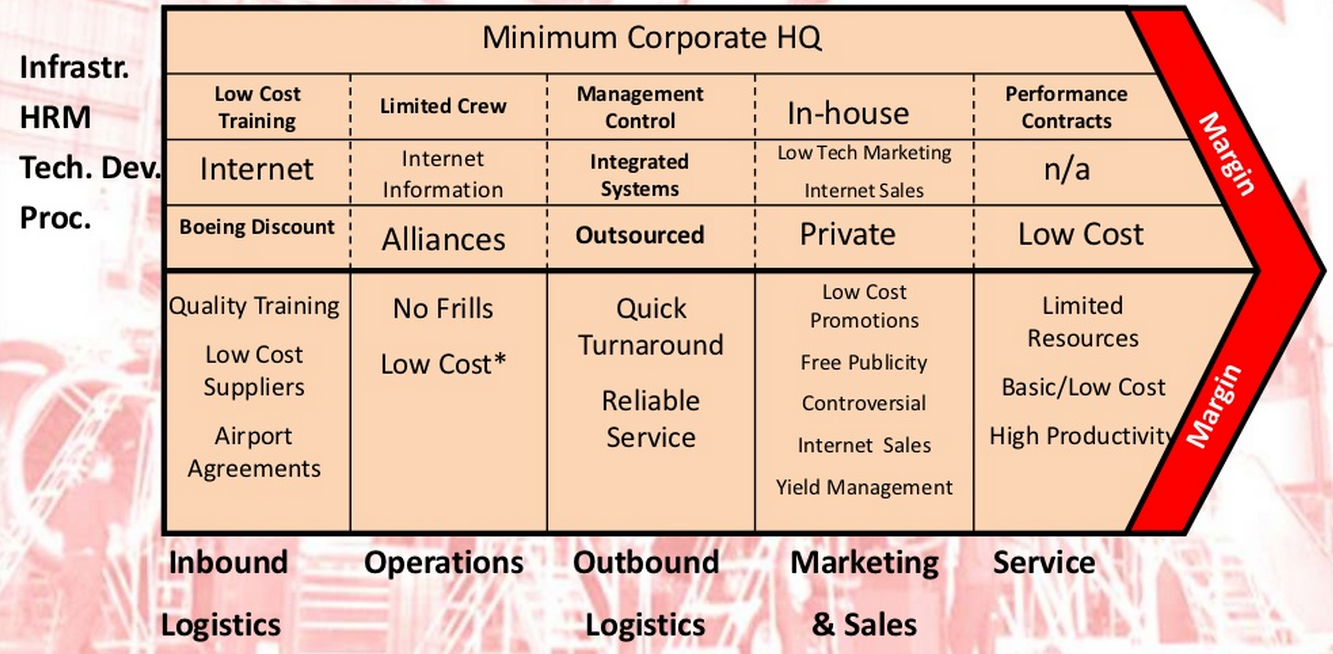
\includegraphics[scale=0.344]{image4}
\end{figure}

Het bovenstaande Value Chain model heb ik gevonden in een presentatie over hoe Ryanair zich competitief heeft opgesteld tegenover de andere luchtvaartmaatschappijen en LCC's. \footnote{http://www.slideshare.net/puya455/newanalysis-of-ryanairs-competitive-advantages \\ slide 7 bevat het Value Chain Model}
\newpage

Deze heb ik gekozen omdat het me echt wel een zeer goede representatie van Ryanair op dit eigenste moment geeft. Ze voorzien zo weinig mogelijk administratief werk, het personeel wordt steeds beperkt tot het minimum en krijgt bonussen naarmate ze meer 'ancillary services' verkopen aan de passagier. Alles verloopt via internet en via outsourcing (bagage-handeling,...) en zo voort voor alle andere dingen.
Het Value Chain Model geeft alle factoren netjes weer en veel van deze dingen die terugkomen,zijn alreeds in deze casestudie vermeld of aangehaald.

\section{Value Chain Network}

Onderstaande Value Chain Network is een voorstelling van hoe de verschillende Value Chains met elkaar om gaan en welke informatie er tussen hen wordt uitgewisseld. Newcomers en substitutes leken me weinig relevant, dus deze heb ik dan ook buiten beschouwing gelaten.

\begin{figure}[h]
\centering
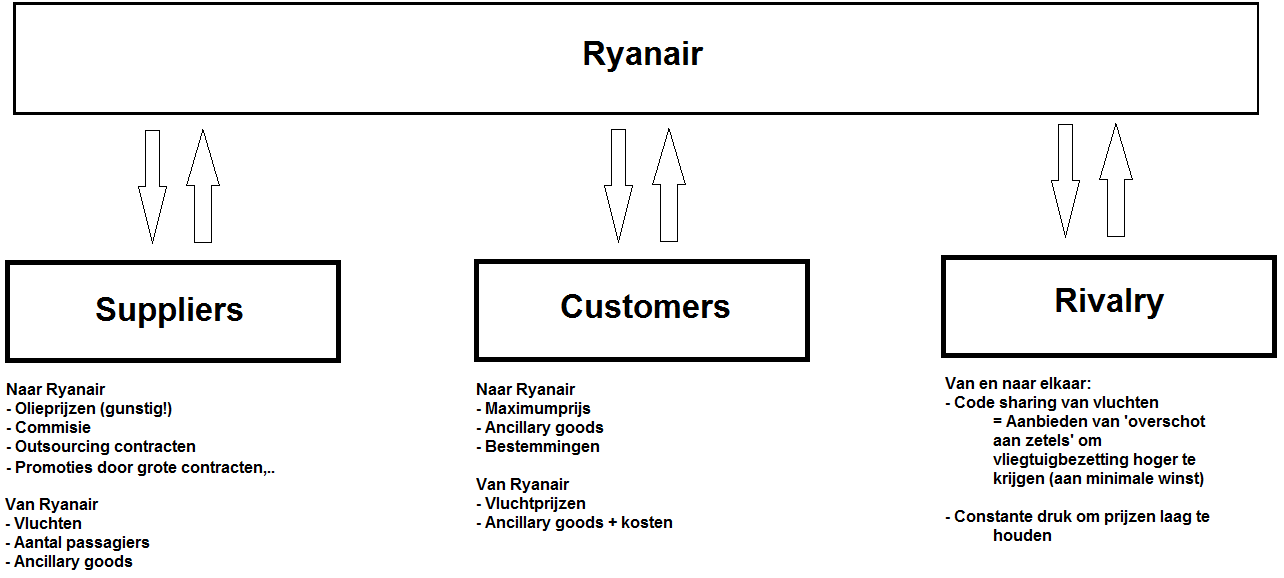
\includegraphics[scale=0.35]{image5}
\end{figure}

\newpage
\part{Imperfecties van de markt}
\setcounter{section}{0}
 \section{De Imperfecties}	
Een markt is nooit perfect. Er zullen altijd een hele resem imperfecties zorgen voor voor- en nadelen. Deze imperfecties kunnen soms grote gevolgen hebben voor alle betrokken partijen, soms ten goede, maar vaak ook ten slechte.
\begin{itemize}
\item Ten eerste hebben we het feit dat de markt niet altijd een uniforme informatie verdeling heeft (Bounded rationality) \\
Hier kunnen we dit duidelijk zien aan de prijzen van de tickets. Een klant weet nog steeds niet wat hij precies betaald. Volgens enkelen ligt de prijs van Ryanair tickets nog steeds veel te hoog, maar door fuel hedging en voordelige contracten met lokale luchthavens/suppliers van ancillary goods, kan deze laag worden gehouden. De klant weet dus niet waarvoor hij eigenlijk betaald.

\item Opportunism is de volgende markt-imperfectie, soms ook wel Information-assymetry genoemd. Ook hier kunnen we weer het voorbeeld van puntje 1 aanhalen. Men weet niet waarvoor men betaald, dus men zal niet kunnen nagaan of er inderdaad een verhoogde brandstof taks is doorgerekend als de prijzen zijn gestegen en hoe de kortingen van een bepaalde promotie in rekening worden gebracht.

\item Als laatste van de imperfecties is er Multi-Interpretable Information, of ook wel informatie die door beide betrokken partijen verschillend ge\"inter-preteerd kan worden. Hiervan zijn vele voorbeelden, maar vooral de vanaf Ryanair uit is dit een voordelige positie. Hotel-ratings, promoties,... niemand kan eigenlijk echt bepalen wat die precies inhouden. De 1-5 sterren rating die voor hotels wordt gebruikt is een puur subjectief beeld van de mensen die er al geweest zijn (mogelijke slechte ervaringen inclusief, terwijl het hotel perfect in orde kan zijn). Enkel diegene die deze ratings, promoties,... maakt heeft en besef van hoe het precies in elkaar zit.
\end{itemize}
\newpage

\section{Solve and Maintain}

Door middel van de Solve en Maintain structuur kunnen bedrijven zichzelf naar een voordeligere positie brengen ten opzichte van klanten en concurrenten. Sommige markt-imperfecties moeten behouden blijven, zodat Ryanair een voordelige deal kan sluiten, een goedkope (maar winstgevende) promotie kan uitschrijven,...

Daarom is het van groot belang dat Ryanair de 3 vermelde imperfecties behandelt. De instandhouding van de eerste twee imperfecties zorgt er voor dat Ryanair meer klanten kan krijgen door met zijn prijzen te spelen en promoties uit te schrijven. De derde imperfectie is van minder groot belang voor Ryanair, maar als hij opgelost kan worden, zou het wel voordelig kunnen uitdraaien voor Ryanair. Betere weergave van hotelratings kan bijvoorbeeld er voor zorgen dat klanten meer combo's kopen (hotel+vlucht), wat extra winst is voor Ryanair.

\newpage
\part{Bronnen}
\begin{itemize}
\item Veelvuldig gebruik van wikipedia: termen, begrippen, informatie over Ryanair, easyJet en andere maatschappijen.
\item Google is uw beste vriend: wederom termen, begrippen en vertalingen.
\item http://www.slideshare.net/puya455/newanalysis-of-ryanairs-competitive-\\advantages, verschillende malen geraadpleegd sinds 1/03/2014
\item http://www.bloomberg.com/news/2014-01-02/ryanair-2013-passenger-\\numbers-rise-2-to-81-4-million-travelers.html, geraadpleegd op 4/03/2014
\item http://www.ryanair.com/en/investor/presentations en alle financi\"ele verslagen (rechter sidebar op de site), verschillende malen geraadpleegd sinds 4/3/2014.
\item http://corporate.easyjet.com/investors/reports-and-accounts.aspx, \\verschillende malen geraadpleegd sinds 4/3/2014.
\item Alle gegeven teksten en verslagen die op TOLEDO zijn verschenen. 
\end{itemize}

\end{document}